\documentclass[11pt]{article}
\usepackage[margin=2.2cm]{geometry}
\usepackage{amsmath,amssymb}
\usepackage{booktabs}
\usepackage{algorithm}
\usepackage[noend]{algpseudocode}
\usepackage{tikz}
\usetikzlibrary{arrows.meta,positioning}
\usepackage[hidelinks]{hyperref}

\newcommand{\x}{\mathbf{x}}
\newcommand{\p}{\mathbf{p}}
\newcommand{\g}{\mathbf{g}}
\newcommand{\ob}{\mathbf{o}}

\title{Radio Flow SLAM\\[2pt]\large How the algorithm works (implementation in \texttt{side\_navlori/dpro/rf})}
\author{}
\date{}

\begin{document}
\maketitle

\section*{1\quad The idea in one paragraph}
The robot records a WiFi scan about every 4\,s (about 0.8\,m of travel): the APs it hears and their signal
strength (RSSI, in dBm). When the robot moves, every AP's signal changes: the AP it drives towards gets
louder, the one behind gets quieter. A physics model turns each change into ``closer'' or ``farther''; we
call these changes \emph{radio flow}, by analogy with optical flow between two images. A solver estimates
the robot path and the AP map together, from radio flow between scans up to 8 apart, from the absolute
RSSI, and from pairs of scans that look like the same place (revisits). Two optional networks help it: one
checks which revisits are real, and one corrects the radio-flow targets and decides how much to trust each
of them. As in DROID-SLAM (Teed and Deng, NeurIPS 2021), the networks never output a position: positions
only come out of the solver. With wheel odometry, the same machinery can also check the odometry.

\begin{center}
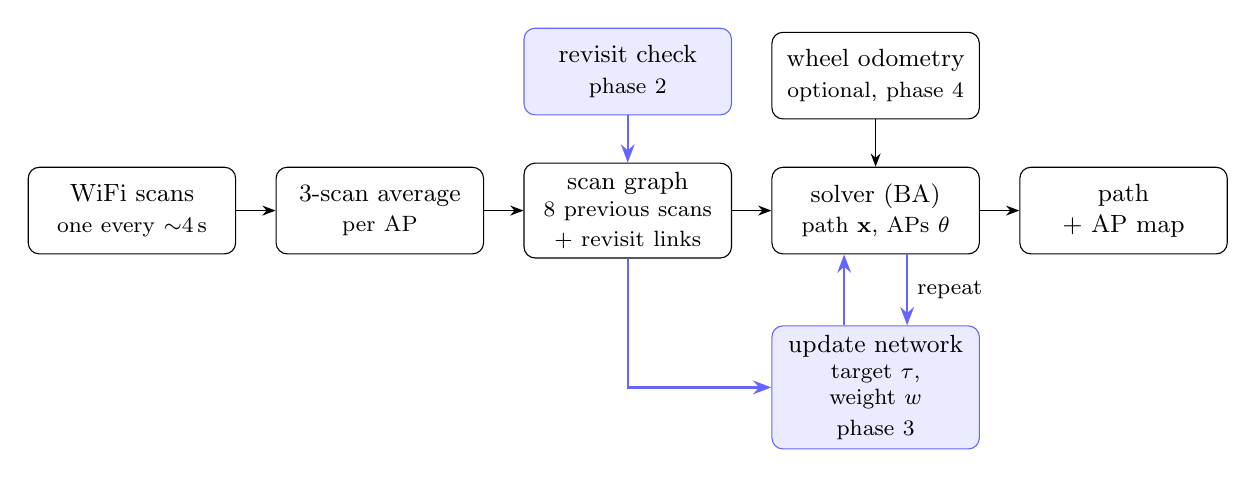
\begin{tikzpicture}[node distance=6mm and 5mm, >=Stealth,
  box/.style={draw, rounded corners, align=center, minimum height=11mm, text width=24mm, font=\small},
  net/.style={box, fill=blue!8, draw=blue!60}]
  \node[box] (scan) {WiFi scans\\ \footnotesize one every $\sim$4\,s};
  \node[box, right=of scan] (avg) {3-scan average\\ \footnotesize per AP};
  \node[box, right=of avg] (graph) {scan graph\\ \footnotesize 8 previous scans\\ + revisit links};
  \node[box, right=of graph] (ba) {solver (BA)\\ \footnotesize path $\x$, APs $\theta$};
  \node[box, right=of ba] (out) {path\\ + AP map};
  \node[net, above=of graph] (rev) {revisit check\\ \footnotesize phase 2};
  \node[net, below=9mm of ba] (nn) {update network\\ \footnotesize target $\tau$, weight $w$\\ phase 3};
  \node[box, above=of ba] (odo) {wheel odometry\\ \footnotesize optional, phase 4};
  \draw[->] (scan) -- (avg); \draw[->] (avg) -- (graph); \draw[->] (graph) -- (ba); \draw[->] (ba) -- (out);
  \draw[->, blue!60, thick] (rev) -- (graph);
  \draw[->] (odo) -- (ba);
  \draw[->, blue!60, thick] (graph.south) |- (nn.west);
  \draw[->, blue!60, thick] ([xshift=-4mm]nn.north) -- ([xshift=-4mm]ba.south);
  \draw[->, blue!60, thick] ([xshift=4mm]ba.south) -- node[right, font=\footnotesize, text=black]{repeat} ([xshift=4mm]nn.north);
\end{tikzpicture}
\end{center}

\section*{2\quad Where it comes from}
Three papers by the same group give the structure: RAFT (optical flow, ECCV 2020) refines a flow field with
a recurrent update operator; DROID-SLAM turns that into SLAM: a graph of frame pairs, a flow revision and a
confidence per pixel, and a differentiable bundle adjustment; DPVO (NeurIPS 2023) keeps the same loop on
sparse patches. DPRO v1 (\texttt{side\_navlori/dpro}) copied DPVO. Radio Flow SLAM copies DROID-SLAM instead,
because a WiFi scan has only $\sim$24 APs: there is no need for patches, every heard AP is used.
\begin{center}\small
\begin{tabular}{@{}ll@{}}
\toprule
DROID-SLAM (camera) & Radio Flow SLAM (WiFi) \\
\midrule
image frame & WiFi scan, averaged over 3 consecutive scans \\
optical flow between frames $i$ and $j$ & radio flow: change of each AP's RSSI between scans $i$ and $j$ \\
correlation volume to find matches & not needed: the AP identity gives the match \\
frame graph: neighbours + proximity edges & links to the 8 previous scans + revisit links \\
unknown depth per pixel (Schur) & unknown AP parameters $\theta_a$, $4\times4$ block per AP (Schur) \\
update operator: flow revision + confidence & target correction $\delta$ (dB) + weight multiplier $e^{z}$ \\
dense bundle adjustment & radio-flow BA + absolute RSSI + motion rules or odometry \\
trained on synthetic TartanAir & trained on synthetic buildings \\
\bottomrule
\end{tabular}
\end{center}

\section*{3\quad Notation, physics model and radio flow}
An AP is one access point on one band; the several networks (BSSIDs) it broadcasts are merged into one,
keeping the strongest reading (24 APs on the golden runs). Scans $j=1,\dots,N$ at times $t_j$; $y_{j,a}$ is
the RSSI of AP $a$ in scan $j$ (missing if not heard). Unknowns: positions $\x_j\in\mathbb{R}^2$ and AP
parameters $\theta_a=(\p_a\in\mathbb{R}^2,P_{0,a},n_a)$. Expected RSSI (log-distance model):
\begin{equation}
h(\x,\theta_a)=P_{0,a}-10\,n_a\log_{10}\!\big(\lVert\x-\p_a\rVert+\varepsilon\big),\qquad\varepsilon=0.5\ \text{m}.
\end{equation}
\paragraph{Radio flow.} The predicted change of AP $a$ between scans $i$ and $j$ is
\begin{equation}
h(\x_j,\theta_a)-h(\x_i,\theta_a)=-10\,n_a\log_{10}\frac{\lVert\x_j-\p_a\rVert+\varepsilon}{\lVert\x_i-\p_a\rVert+\varepsilon}.
\end{equation}
The AP's power $P_{0,a}$ cancels, and so does any constant gain of the phone: only the ratio of the two
distances matters. This is what radio flow was meant to buy. (In an absolute model with a free $P_{0,a}$,
the solver already uses changes implicitly; radio flow makes them explicit and lets each link carry its
own noise level.)

\paragraph{3-scan averages.} Each reading is replaced by its centred average over scans $j-1,j,j+1$:
$\bar y_{j,a}=\frac{1}{c_{j,a}}\sum_{j'=j-1}^{j+1}y_{j',a}$ over the $c_{j,a}$ scans that heard $a$, kept
only if $c_{j,a}\ge2$. On the golden runs this cuts the noise of a change between scans 2 apart from 5.6 to 3.3\,dB. It needs scan
$j+1$, so scan $j$ is estimated one scan ($\sim$4\,s) late.

\section*{4\quad The scan graph}
\begin{center}
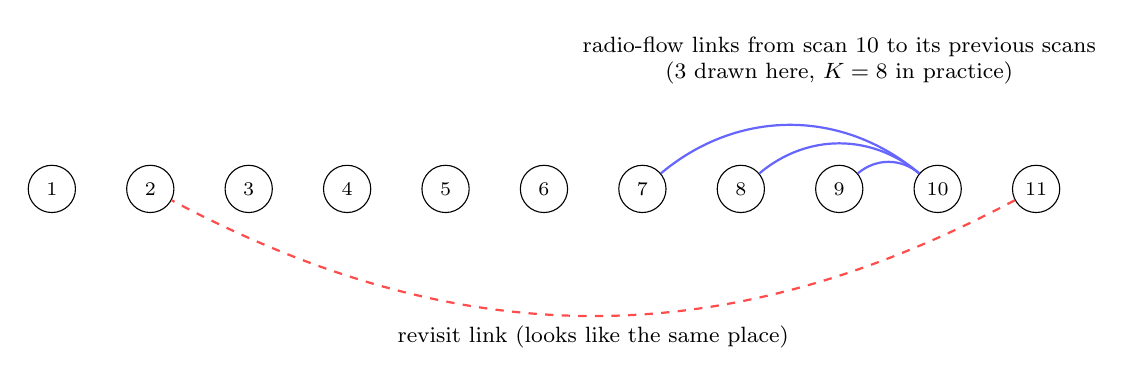
\begin{tikzpicture}[>=Stealth, scan/.style={circle, draw, fill=white, inner sep=1.5pt, font=\scriptsize, minimum size=6mm}]
  \foreach \i in {1,...,11} \node[scan] (s\i) at (1.25*\i,0) {\i};
  \foreach \k in {7,8,9} \draw[blue!60, thick] (s10) to[bend right=40] (s\k);
  \draw[red!70, thick, dashed] (s11) to[bend left=28] node[below, font=\footnotesize, text=black]{revisit link (looks like the same place)} (s2);
  \node[font=\footnotesize, align=center, above=9mm of s9] {radio-flow links from scan 10 to its previous scans\\ (3 drawn here, $K=8$ in practice)};
\end{tikzpicture}
\end{center}
Three kinds of factors, each per AP heard in the scans involved:
\begin{itemize}
\item \textbf{Radio-flow factor} $(i,j,a)$, $j-8\le i<j$: measured change $\Delta y_{ij,a}=\bar y_{j,a}-\bar y_{i,a}$,
residual $r=\Delta y_{ij,a}-\big(h(\x_j,\theta_a)-h(\x_i,\theta_a)\big)$.
\item \textbf{Absolute factor} $(j,a)$: residual $r=\bar y_{j,a}-h(\x_j,\theta_a)$.
\item \textbf{Revisit factor} $(i,j,a)$: same residual as radio flow, for scan pairs proposed as the same place.
\end{itemize}

\paragraph{Revisit proposals} (DROID-SLAM's proximity edges). Fingerprint distance between two scans:
$D_{ij}=\big(\frac1L\sum_a(\tilde y_{i,a}-\tilde y_{j,a})^2\big)^{1/2}$, with unheard APs set to $-100$\,dBm.
Candidates are pairs at least 7 scans apart, taken from the smallest $D_{ij}$ up; each taken pair suppresses
its neighbours within $\pm2$ scans (non-maximum suppression); at most $\lfloor N/6\rfloor$ pairs per run.

\section*{5\quad Noise model and weights}
Real-data checks split the RSSI error into a random part ($\sigma_n=3.5$\,dB per reading) and a
place-dependent part ($\sigma_s=5.0$\,dB) that stays the same over $\ell=3.5$\,m. Two scans $d$ metres apart
share part of the place-dependent error, so their change is cleaner:
\begin{align}
\sigma^2_{\text{flow}}(i,j,a)&=\sigma_n^2\Big(\frac{1}{c_{i,a}}+\frac{1}{c_{j,a}}\Big)+2\sigma_s^2\big(1-e^{-d_{ij}/\ell}\big),\\
\sigma^2_{\text{abs}}(j,a)&=\frac{\sigma_n^2}{c_{j,a}}+\sigma_s^2 ,
\end{align}
where $d_{ij}=0.8\,\text{m}\times(j-i)$ for temporal links and 1\,m for revisit links. Each factor's weight is $w=c_{\text{type}}/\sigma^2$, with one multiplier per factor type chosen on 24
synthetic buildings only (never on the real runs). Best combination: $c_{\text{flow}}=0.03$,
$c_{\text{abs}}=1$, $c_{\text{rev}}=1$ (radio flow alone: $c_{\text{flow}}=0.3$).

\paragraph{Robust revisits.} A wrong revisit pulls two distant scans together. For each proposed pair $e$,
let $\rho_e$ be the RMS of the normalised residuals $\sqrt{w}\,r$ over its APs. Its weights are scaled by
$s_e=1/\big(1+(\rho_e/2)^2\big)$ (Cauchy), recomputed at each of the final solver steps (iteratively
reweighted least squares).

\section*{6\quad The solver}
The solver minimises
\begin{align}
\mathcal{E}(\x,\theta)=\;&\sum_{\text{flow}}w\,r^2+\sum_{\text{abs}}w\,r^2+\sum_{e}\sum_{\text{rev}\in e}s_e\,w\,r^2
&&\text{WiFi}\nonumber\\
&+\sum_{j}\left\lVert\frac{\x_{j+1}-2\x_j+\x_{j-1}}{\sigma_{\text{acc}}}\right\rVert^2
&&\text{smoothness (without odometry)}\nonumber\\
&+\sum_{j}\left(\frac{\lVert\x_{j+1}-\x_j\rVert-v_0\Delta t_j}{\sigma_v\Delta t_j}\right)^{\!2}
&&\text{speed (without odometry)}\nonumber\\
&+\sum_a\left[\left(\frac{P_{0,a}-\bar P_0}{\sigma_P}\right)^{\!2}+\left(\frac{n_a-\bar n}{\sigma'_n}\right)^{\!2}\right]
&&\text{weak AP priors}
\end{align}
with $\sigma_{\text{acc}}=0.3$\,m, $v_0=0.2$\,m/s, $\sigma_v=0.1$\,m/s (both from DPRO v1: WiFi alone cannot
see scale), $\bar P_0=-40$\,dBm, $\sigma_P=15$\,dB, $\bar n=3$, $\sigma'_n=1$; after each step $n_a$ is kept in
$[1.5,6]$ and $P_{0,a}$ in $[-90,-10]$\,dBm.

\paragraph{One Gauss--Newton step.} Each factor touches at most two positions and one AP. The normal equations
\begin{equation}
\begin{bmatrix} B & E\\ E^\top & C\end{bmatrix}\begin{bmatrix}\Delta\x\\ \Delta\theta\end{bmatrix}=\begin{bmatrix} v\\ u\end{bmatrix}
\end{equation}
have a block-diagonal $C$ (one $4\times4$ block per AP), so the APs are eliminated by a Schur complement:
\begin{equation}
\big(B-EC^{-1}E^\top\big)\Delta\x=v-EC^{-1}u,\qquad \Delta\theta=C^{-1}\big(u-E^\top\Delta\x\big),
\end{equation}
with Levenberg--Marquardt damping (0.1 on the positions, $10^{-3}$ on the AP blocks). The first 3 positions
are fixed (the gauge). Every operation is differentiable, so a loss on the positions can train the network
of Section 9 through the solver.

\paragraph{New APs.} An AP heard for the first time is placed at the scan where it is strongest, plus a
random offset ($\mathcal{N}(0,2^2)$\,m per axis; this offset is what the evaluation seeds change), with
$n_a=3$ and $P_{0,a}$ set so that its strongest reading sits 2.5\,m away.

\section*{7\quad Running on a recording}
\begin{algorithm}[h]
\caption{Radio Flow SLAM, one scan at a time (frontend), then one global solve (backend)}
\begin{algorithmic}[1]
\For{each scan $j$ (its 3-scan average is available once scan $j+1$ arrives)}
  \State $\x_j\gets\x_{j-1}+\tfrac12\,\tfrac{t_j-t_{j-1}}{t_{j-1}-t_{j-2}}(\x_{j-1}-\x_{j-2})$ \Comment{damped constant velocity}
  \State initialise the APs heard for the first time (Section 6)
  \State add radio-flow factors to scans $j-8,\dots,j-1$ and absolute factors for scan $j$
  \If{$j=8$} 12 solver steps on all positions \Comment{start-up}
  \ElsIf{$j>8$} 3 solver steps on the last 12 positions \Comment{older ones frozen}
    \State (phase 3, online variant: 2 learned updates)
  \EndIf
  \State record $\x^{\text{causal}}_j\gets\x_j$ \Comment{the estimate a robot would have now}
\EndFor
\State propose revisit pairs (Section 4) and add their factors
\State 12 solver steps on all positions, recomputing the robust revisit weights $s_e$ before each
\State (phase 3: 12 learned updates, Section 9)
\end{algorithmic}
\end{algorithm}

\section*{8\quad Learned revisit check (phase 2)}
A small network gives the probability that scans $i$ and $j$ were taken less than 3\,m apart. It never sees
AP identities, so it can run in a new building. For each AP heard in either scan it reads 8 values: both
raw readings and both 3-scan averages (scaled as $(y+70)/15$, 0 if not heard), two heard flags, the absolute
difference if heard in both, and the larger of the two readings. An MLP ($8\to48\to48$) embeds each AP; mean
and max pooling over the APs are concatenated with 6 pair features (APs shared, APs heard in either, their
ratio, mean difference over shared APs, $D_{ij}$, difference in number of APs heard), and an MLP gives the logit.
Training: binary cross-entropy weighted for the rare positives, 3000 steps of 256 pairs, AdamW ($10^{-3}$),
on 150 synthetic buildings (3 runs of 30 scans each; all near pairs, the most look-alike far pairs, random far
pairs). A variant adds the real pairs of the other zone (held out by zone). Optionally, scores are averaged
over 3 consecutive pairs in the same or the opposite direction (sequence matching, as SeqSLAM). With learned
scores $p_{ij}$, proposals are taken from the highest $p_{ij}$ and each revisit weight is multiplied by $p_{ij}$.

\section*{9\quad Learned update operator (phase 3)}
One hidden state $z_f\in\mathbb{R}^{64}$ per radio-flow or revisit factor $f=(i,j,a)$. Its 17 inputs: the
measured change and both averaged readings; $1/c_{i,a}$, $1/c_{j,a}$; the predicted change, the residual and
the previous iteration's residual; $\log(d_{i,a}+0.5)$, $\log(d_{j,a}+0.5)$ with $d$ the current distance to the
AP; $P_{0,a}$, $n_a$; scans apart; temporal or revisit; the revisit score; $D_{ij}$; number of shared APs.
One update (as DROID-SLAM's operator, without correlation features):
\begin{enumerate}
\item $z_f\gets\mathrm{LayerNorm}\big(z_f+\mathrm{MLP}(\text{inputs}_f)\big)$;
\item add soft aggregations over the factors of the same scan pair, of the same AP, and of the same scan $j$;
\item two gated residual layers;
\item two heads, both initialised to zero:
\begin{equation}
\tau_f=\Delta y_f+10\,\delta_f\ \text{dB},\qquad w_f=w^{\text{hand}}_f\,e^{z_f'},\quad z_f'\in[-5,2],
\end{equation}
\item 2 solver steps with the radio-flow targets $\tau_f$ and weights $w_f$ (absolute factors keep their hand weights).
\end{enumerate}
Because both heads start at zero, an untrained network reproduces the hand-weighted solver exactly; the
target is anchored on the measurement, not on the model.

\begin{algorithm}[h]
\caption{One training step (DROID-SLAM's recipe on synthetic buildings)}
\begin{algorithmic}[1]
\State new synthetic building, one 32-scan run (true positions $\g_j$, noise-free RSSI known)
\State run the hand-weighted solver (Algorithm 1, no gradient): start $\x^{(0)},\theta^{(0)}$
\For{$s=1,\dots,6$}
  \State update (network + 2 solver steps), gradients flow through the solver
  \State $\mathcal{L}^{(s)}_{\text{pose}}=\frac1N\sum_j\lVert R\x_j+\mathbf{t}-\g_j\rVert$ \Comment{best rigid fit, mirror allowed}
  \State $\mathcal{L}^{(s)}_{\text{flow}}=\text{mean}_f\,|\tau_f-\Delta y^{\text{true}}_f|/5$
\EndFor
\State $\mathcal{L}=\sum_s0.9^{\,6-s}\big(\mathcal{L}^{(s)}_{\text{pose}}+0.1\,\mathcal{L}^{(s)}_{\text{flow}}\big)$; AdamW ($3\cdot10^{-4}$, one-cycle), gradient clip 10
\end{algorithmic}
\end{algorithm}
1500 steps ($\sim$30\,min on one CPU core), 3 independent trainings. Two ways to run it: 12 learned updates
after the run, or also 2 after each scan (online).

\section*{10\quad With wheel odometry (phase 4)}
\paragraph{Odometry factor.} The motion rules are replaced by the odometry steps $\ob_j$ (in the odometry's own frame):
\begin{equation}
\sum_j\frac{\big\lVert(\ob_{j+1}-\ob_j)-(\x_{j+1}-\x_j)\big\rVert^2}{\sigma_{o,j}^2},\qquad
\sigma_{o,j}=0.05\ \text{m}+0.05\,\lVert\ob_{j+1}-\ob_j\rVert .
\end{equation}
Only the first position is fixed; new positions start at $\x_{j-1}+(\ob_j-\ob_{j-1})$. The radio-flow multiplier
was retuned on synthetic runs with simulated odometry ($c_{\text{flow}}=0.1$).

\paragraph{WiFi gyro-bias check.} On two golden runs the robot's \texttt{/odom} heading (integrated gyro) turns at
a constant wrong rate $b$. One unknown per run, so it is searched directly. For a candidate $b$ the odometry
steps are un-rotated,
\begin{equation}
\ob^{\,b}_{j+1}=\ob^{\,b}_j+\mathrm{Rot}(-b\,\bar t_j)\,(\ob_{j+1}-\ob_j),\qquad \bar t_j=\tfrac12(t_j+t_{j+1})-t_1,
\end{equation}
and the path is scored by how well it explains the RSSI: for each AP, over a grid of positions $\p$ (0.75\,m
cells, path $\pm10$\,m), $P_0$ and $n$ are fitted in closed form ($n$ kept in $[1,6]$), and the best robust misfit is kept,
\begin{equation}
c(b)=\frac{1}{n_{\text{readings}}}\sum_a\min_{\p}\sum_j\rho\big(y_{j,a}-\hat h_a(\ob^{\,b}_j;\p)\big),\qquad
\rho(r)=f^2\Big(\sqrt{1+(r/f)^2}-1\Big),\ f=4\ \text{dB}.
\end{equation}
A curled path explains the RSSI badly. $b^\star$ is found on a grid ($-30$ to $30\,^\circ$/s by 1, then $\pm1$ by 0.1),
and the correction is kept only if $c(0)/c(b^\star)>1.3$. The margin 1.3 was chosen on 48 synthetic runs (12--60
scans, half with a bias of 2--25\,$^\circ$/s). The online version re-estimates $b$ at every scan from the scans so far.

\paragraph{Control: wheel encoders only.} Dead reckoning from the wheel angles $\varphi_L,\varphi_R$, no gyro:
$\Delta s=r_w(\Delta\varphi_R+\Delta\varphi_L)/2$, $\Delta\psi=r_w(\Delta\varphi_R-\Delta\varphi_L)/B$, with
$r_w=0.033$\,m, $B=0.287$\,m, integrated at the mid-step heading.

\section*{11\quad Evaluation}
Scores per run (median over its scans), then the mean over the 12 golden runs:
\begin{itemize}
\item \textbf{aligned}: $\lVert R\x_j+\mathbf{t}-\g_j\rVert$ after the best rigid fit of the whole path (mirror allowed), as in the literature;
\item \textbf{causal}: the same, on $\x^{\text{causal}}_j$, each scan as it was first estimated;
\item \textbf{online}: $R,\mathbf{t}$ fitted on the first 30\,s only, error on the rest (for WiFi alone this mostly
measures how the map is turned: the robot moves only 0.7--5.4\,m in those 30\,s);
\item \textbf{drift per 5\,m}: $\lVert R(\x_{j'}-\x_j)-(\g_{j'}-\g_j)\rVert$, with $j'$ the first scan 5\,m of travel after $j$.
\end{itemize}
Weights and thresholds come from synthetic data only; 3 evaluation seeds; 3 trainings for the learned parts.
``Ceiling'' rows use the truth (true AP map, true gyro bias) and are limits, not methods.

\section*{12\quad Results on the 12 golden runs}
\begin{center}\small
\begin{tabular}{@{}lrrr@{}}
\toprule
method & aligned (m) & causal (m) & drift per 5\,m (m) \\
\midrule
motion rules only (no WiFi) & 3.57 & 3.65 & 3.70 \\
DPRO v1, network off, tuned (best earlier method) & 1.47 & 2.23 & 2.09 \\
radio flow, single scans & 1.59 & 2.23 & 2.25 \\
radio flow, 3-scan average & 1.74 & 2.57 & 2.26 \\
absolute RSSI only & 1.46 & 2.27 & 2.10 \\
radio flow + absolute + revisits (best hand-weighted) & 1.47 & 2.18 & 2.19 \\
learned update, after the run (3 trainings) & 1.52 & 2.18 & 2.10 \\
learned update, also online (3 trainings) & 1.46 & 2.08 & 1.97 \\
ceiling: absolute RSSI with the true AP map & 1.20 & 1.68 & 1.83 \\
\midrule
\texttt{/odom} (gyro heading) & 0.48 & 0.48 & 0.57 \\
\texttt{/odom} + radio flow & 0.48 & 0.49 & 0.56 \\
\texttt{/odom} after the WiFi gyro-bias check & 0.30 & 0.48 & 0.33 \\
wheel encoders only, no gyro & 0.13 & 0.13 & 0.14 \\
\bottomrule
\end{tabular}
\end{center}
WiFi alone ties the best earlier method; the true AP map would gain only 0.27\,m, so the RSSI noise, not the
map, is the limit here. Learned revisit proposals are within 3\,m 30--32\,\% of the time (raw: 25\,\%; best
possible at that count: 61\,\%). The learned update beats the hand weights on 21--25 of 30 new synthetic
buildings but gains only 0.02\,m on the real runs. The WiFi gyro-bias check fixes run 4 (2.55\,$\to$\,0.34\,m),
but the wheel encoders, which do not share the gyro's fault, do better without WiFi.

\end{document}
